\chapter{Analyse et spécification des besoins}

\section*{Introduction}

\qquad Après avoir présenté le contexte général de notre projet, nous venons d’énoncer dans cette partie les besoins auxquels notre application devra réponde. Nous énumérerons les besoins fonctionnels et non fonctionnels dans une première partie et nous exposerons par la suite la spécification de ces besoins à travers les diagrammes de cas d’utilisation.

\section{Analyse des besoins}

\qquad Ce chapitre est dédié à l'étude profonde des différents besoins sur l'échelle fonctionnelle et non fonctionnelle. Nous projetons de détailler les risques et contraintes auxquelles est soumis notre projet dans le but de répondre aux besoins.

\subsection{Identification des acteurs}

\qquad L'application doit garantir la prévention contre les risques de pollution pour l'utilisateur final et la suivi et contrôle pour les administrateurs de Smartdata.

\subsection{Besoins fonctionnels}
\qquad Nous présentons ci-dessous les besoins fonctionnels regroupés par acteur:

\begin{itemize}
	\item Utilisateur
		\begin{itemize}
			\item Visualisation des niveaux des risques
			\item Inscription aux différents risques
			\item Visualisation des détails sur les risques
			\item Visualisation des états des stations
			\item Visualisation des conseils
			\item Inscription aux rappels santé
			\item Ajout d'astuces
		\end{itemize}
	\item Administrateur
		\begin{itemize}
			\item Consultation des statistiques
			\item Réception des Emails concernant les batchs
			\item Réception des Emails concernant les notifications
		\end{itemize}
\end{itemize}

\subsection{Besoins non fonctionnels}

\qquad Pour bien répondre à ses besoins notre application doit respecter les exigences techniques suivantes: 

\textbf{Ergonomie} Le but de l’application est qu’elle soit exploitée par des simples utilisateurs qui ne sont pas forcément expérimentés dans le domaine de l’informatique, et qu’elle le soit de la façon la plus efficace. Les interfaces de l’application doivent être ergonomiques et conviviales.

\textbf{Environnement et architecture} L’application doit être mise en place dans une architecture répartie multi-tiers et accessible via le Web à travers les navigateurs Web.

\textbf{Rapidité} Notre application doit garantir un accès rapide aux données et d’une manière transparente.

\textbf{Scalabilité} L’application doit être facilement extensible pour pouvoir accueillir un public plus large.

\textbf{Documentation} L’application sera livrée avec une documentation des différentes fonctions et API qu’elle offre, nécessaire pour les futurs développeur

\section{Spécification des besoins}

\qquad Dans ce paragraphe, nous allons préciser les différents besoins de notre application en ayant recours au langage de modélisations UML. Nous illustrons les besoins par les diagrammes de cas d'utilisation.

\subsection{Diagramme de cas d'utilisation global}

\qquad Nous présentons dans cette partie le diagramme de cas d'utilisation global de notre application. La figure \ref{fig2.1} représente le diagramme de cas d'utilisation global.

\begin{figure}[!h]

	\begin{center}
		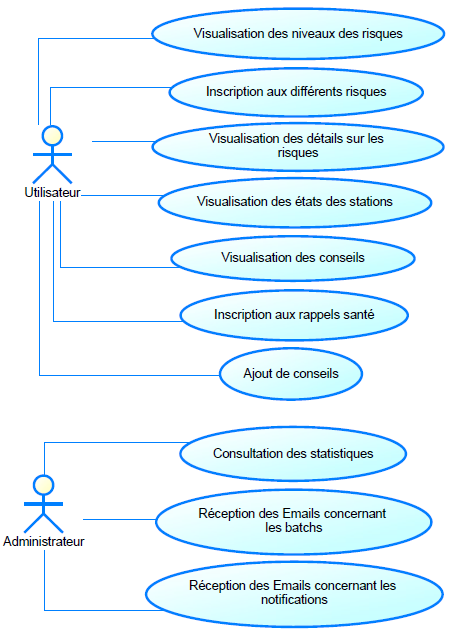
\includegraphics[width =7.1cm ]{figures/globalusecase}		
	\end{center}
	\caption{Diagramme des cas d'utilisation global}
	\label{fig2.1}
\end{figure}

\subsection{Raffinement des cas d'utilisation}

\qquad Dans cette partie, nous présentons les diagrammes de cas d'utilisation raffinés. Nous détaillerons quelques cas d'utilisation parmi ceux qui sont précédemment présentés. 

\subsubsection{Cas d'utilisation : Ajouter astuces}

\qquad La figure \ref{fig2.2} représente le diagramme de cas d'utilisation de l'ajout des astuces.

\begin{figure}[!h]
	\begin{center}
		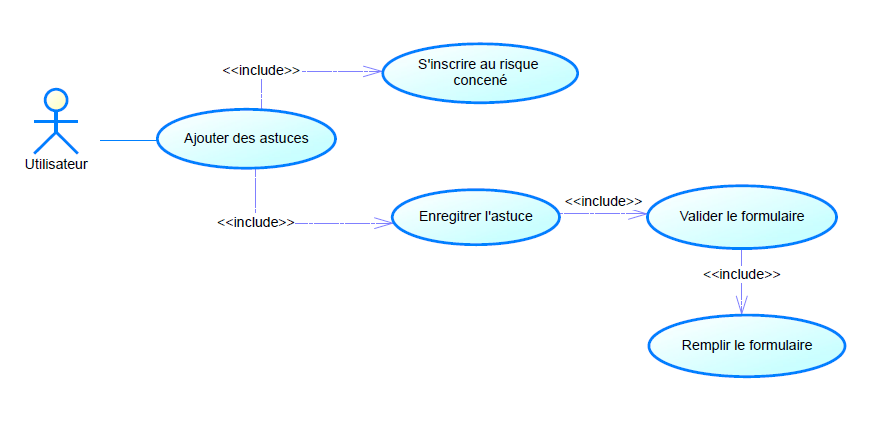
\includegraphics[width=0.64\textheight]{figures/uc_ajoutastuce}
	\end{center}
	\caption{Cas d'utilisation : Ajouter des astuces}
	\label{fig2.2}
\end{figure}

Ci-dessous une description sous forme de tableau du cas d'utilisation : Ajouter astuce.

\begin{table}[!h]
	\caption{Description textuelle du cas d'utilisation : Ajouter astuce}
	\begin{center}
		\begin{tabular}{|L{4cm}|L{10cm}|}
			\hline
			\textbf{Cas d’utilisation} & Ajouter astuce\\
			\hline
			\textbf{Objectif} & Permettre d'ajouter des astuces\\
			\hline
			\textbf{Acteur} & Utilisateur\\
			\hline
			\textbf{Pré-conditions} & S'inscrire, remplir et valider le formulaire\\
			\hline
			\textbf{Post-condition} & Astuce ajoutée\\
			\hline			
			\textbf{Scénarios nominaux} & \textbf{S1. Soumettre une astuce} L'utilisateur remplie le formulaire d'ajout d'astuces, choisit le type de risque, saisit son adresse électronique enfin il confirme l'ajout par cliquer sur le bouton enregistrer\\
			\hline
			\textbf{Exceptions} & \textbf{E1} Utilisateur non inscrit au risque.\\ &\textbf{E2} L'un des champs du formulaire est soit vide soit non valide.\\
			\hline
		\end{tabular}
	\end{center}
\end{table}
 
\subsubsection{Cas d'utilisation : visualisation des niveaux des risques}
\qquad Cette partie est consacrée au raffinement du cas d'utilisation : visualisation des niveaux des risques. La figure \ref{fig2.3} représente en détail le cas d'utilisation avec son acteur et ses pré-conditions.\\

\begin{figure}[!h]
	\begin{center}
		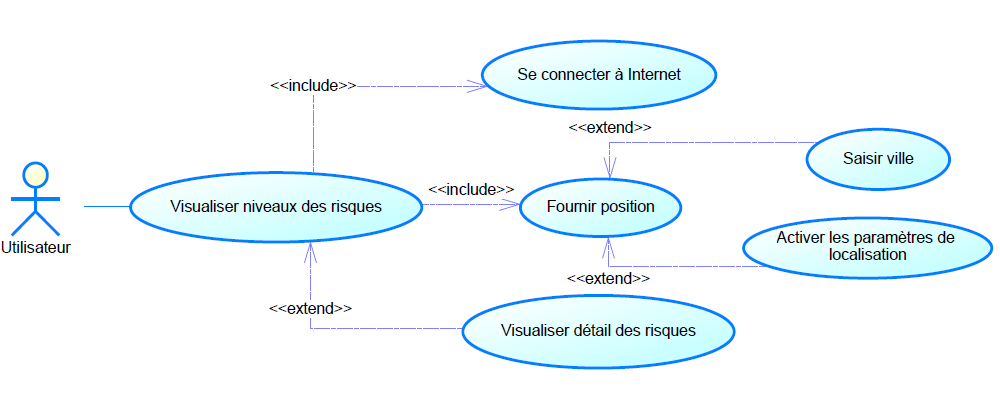
\includegraphics[width=0.64\textheight]{figures/uc_visualisationrisques}
	\end{center}
	\caption{Cas d'utilisation :  visualisation des niveaux des risques}
	\label{fig2.3}
\end{figure}
Le tableau ci-après est une description textuelle du cas d'utilisation.
\begin{table}[!h]
	\caption{Description textuelle du cas d'utilisation : visualiser les niveaux des risques}
	\begin{center}
		\begin{tabular}{|L{4cm}|L{10cm}|}
			\hline
			\textbf{Cas d’utilisation} & visualiser les niveaux des risques\\
			\hline
			\textbf{Objectif} & Permettre de consulter les niveaux des risques\\
			\hline
			\textbf{Acteur} & Utilisateur\\
			\hline
			\textbf{Pré-conditions} & S'inscrire, saisir ville, activer la géolocalisation, se connecter à Internet\\
			\hline
			\textbf{Post-condition} & Niveaux des risques consultés \\
			\hline			
			\textbf{Scénarios nominaux} & \textbf{S1. Consulter le niveau des risques} L'utilisateur se connecte à internet et fournit la ville qu'il veut consulter en saisissant la ville ou en activant le système GPS. Il recevra ainsi le niveaux de risques de la ville souhaitée.\\
			&\textbf{S2} Après avoir reçu les niveaux de risque, l'utilisateur peut consulter les détails sur chaque risque (polluant)\\
			\hline
			\textbf{Exceptions} & \textbf{E1} Utilisateur non inscrit au risque.\\ &\textbf{E2} Téléphone non connecté à Internet\\
			&\textbf{E3} Ville non fourni et système GPS non activé\\
			\hline
		\end{tabular}
	\end{center}
\end{table}
\section*{Conclusion}
\qquad Nous avons consacré ce chapitre, à la spécification des besoins, ce qui permet de mieux comprendre les problématiques soulevées et d’avoir une vue globale sur les fonctionnalités constituantes notre projet. Nous nous intéressons dans le chapitre suivant aux éléments de conception basée sur le travail effectué dans le présent chapitre.